% This file was created with tikzplotlib v0.10.1.
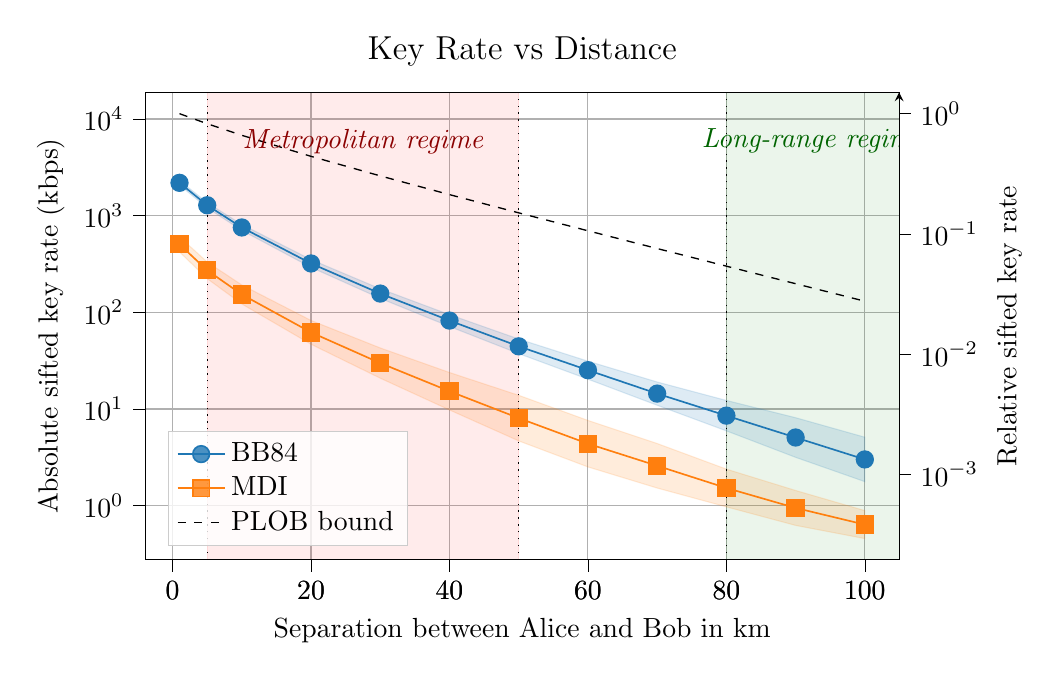
\begin{tikzpicture}
\definecolor{darkgray176}{RGB}{176,176,176}
\definecolor{darkgreen}{RGB}{0,100,0}
\definecolor{darkorange25512714}{RGB}{255,127,14}
\definecolor{darkred}{RGB}{139,0,0}
\definecolor{dimgray}{RGB}{105,105,105}
\definecolor{green}{RGB}{0,128,0}
\definecolor{lightgray204}{RGB}{204,204,204}
\definecolor{steelblue31119180}{RGB}{31,119,180}
\begin{axis}[
width=0.92\linewidth,
height=0.62\linewidth,
legend cell align={left},
legend pos=south west,
legend style={fill opacity=0.8, draw opacity=1, text opacity=1, draw=lightgray204, font=\fontsize{10}{12}\selectfont},
log basis y={10},
tick align=outside,
tick pos=left,
tick label style={font=\fontsize{10}{12}\selectfont},
label style={font=\fontsize{10}{12}\selectfont},
title style={font=\fontsize{12}{14}\selectfont},
x grid style={darkgray176},
xlabel={Separation between Alice and Bob in km},
xmajorgrids,
xmin=-3.95, xmax=104.95,
xtick style={color=black},
xtick={-20,0,20,40,60,80,100,120},
xticklabels={
  \(\displaystyle {\ensuremath{-}20}\),
  \(\displaystyle {0}\),
  \(\displaystyle {20}\),
  \(\displaystyle {40}\),
  \(\displaystyle {60}\),
  \(\displaystyle {80}\),
  \(\displaystyle {100}\),
  \(\displaystyle {120}\)
},
y grid style={darkgray176},
ylabel={Absolute sifted key rate (kbps)},
ymajorgrids,
ymin=0.275385950295772, ymax=18833.9022192978,
ymode=log,
ytick style={color=black},
ytick={0.01,0.1,1,10,100,1000,10000,100000,1000000},
yticklabels={
  \(\displaystyle {10^{-2}}\),
  \(\displaystyle {10^{-1}}\),
  \(\displaystyle {10^{0}}\),
  \(\displaystyle {10^{1}}\),
  \(\displaystyle {10^{2}}\),
  \(\displaystyle {10^{3}}\),
  \(\displaystyle {10^{4}}\),
  \(\displaystyle {10^{5}}\),
  \(\displaystyle {10^{6}}\)
}
]
\path [draw=red, fill=red, opacity=0.08]
(axis cs:5,0.275385950295772)
--(axis cs:5,18833.9022192978)
--(axis cs:50,18833.9022192978)
--(axis cs:50,0.275385950295772)
--cycle;
\path [draw=green, fill=green, opacity=0.08]
(axis cs:80,0.275385950295772)
--(axis cs:80,18833.9022192978)
--(axis cs:104.95,18833.9022192978)
--(axis cs:104.95,0.275385950295772)
--cycle;
\path [draw=steelblue31119180, fill=steelblue31119180, opacity=0.15]
(axis cs:1,2306.62552475261)
--(axis cs:1,2072.52714625355)
--(axis cs:5,1205.13822580594)
--(axis cs:10,703.812107099486)
--(axis cs:20,292.147989278819)
--(axis cs:30,139.585244217195)
--(axis cs:40,71.3906022821082)
--(axis cs:50,37.4310624606331)
--(axis cs:60,20.3684103866127)
--(axis cs:70,10.9430953522866)
--(axis cs:80,5.94404219080003)
--(axis cs:90,3.16365372154705)
--(axis cs:100,1.77327960355882)
--(axis cs:100,5.11189819527521)
--(axis cs:100,5.11189819527521)
--(axis cs:90,8.1375748505655)
--(axis cs:80,12.2672521967809)
--(axis cs:70,19.0472731285524)
--(axis cs:60,31.2649982666408)
--(axis cs:50,52.9763790309403)
--(axis cs:40,94.7320495846122)
--(axis cs:30,175.259425418369)
--(axis cs:20,351.459386200178)
--(axis cs:10,810.523048220432)
--(axis cs:5,1363.99247958231)
--(axis cs:1,2306.62552475261)
--cycle;
\path [draw=darkorange25512714, fill=darkorange25512714, opacity=0.15]
(axis cs:1,604.324126790368)
--(axis cs:1,422.245168341707)
--(axis cs:5,223.260552145066)
--(axis cs:10,122.120435559709)
--(axis cs:20,46.750634028275)
--(axis cs:30,20.8387199399906)
--(axis cs:40,9.78121461724959)
--(axis cs:50,4.68117108894463)
--(axis cs:60,2.51843595191845)
--(axis cs:70,1.52315025946615)
--(axis cs:80,0.972720285955346)
--(axis cs:90,0.625448576336337)
--(axis cs:100,0.456787741032355)
--(axis cs:100,0.889916134566001)
--(axis cs:100,0.889916134566001)
--(axis cs:90,1.43695159988299)
--(axis cs:80,2.38966419063619)
--(axis cs:70,4.39744323842224)
--(axis cs:60,7.62262101278499)
--(axis cs:50,13.8688126026783)
--(axis cs:40,23.8722030869459)
--(axis cs:30,42.8507818302899)
--(axis cs:20,82.4531781575873)
--(axis cs:10,191.996325701147)
--(axis cs:5,331.697783129057)
--(axis cs:1,604.324126790368)
--cycle;
\addplot [semithick, steelblue31119180, mark=*, mark size=3, mark options={solid}]
table {%
1 2186.44552099775
5 1282.1074357699
10 755.28533311638
20 320.434319309823
30 156.408534608532
40 82.2373277488028
50 44.5304631959438
60 25.2352593692174
70 14.4373171346617
80 8.53914894019598
90 5.07390076374767
100 3.01078474905641
};
\addlegendentry{BB84}
\addplot [semithick, darkorange25512714, mark=square*, mark size=3, mark options={solid}]
table {%
1 505.146456633672
5 272.130538908605
10 153.123071156792
20 62.086539253799
30 29.8823600435282
40 15.2806787080936
50 8.05743660190068
60 4.38144756974755
70 2.58804304631714
80 1.52462285003632
90 0.948018635054732
100 0.637575705949223
};
\addlegendentry{MDI}
\addplot [line width=0.48pt, black, dotted, forget plot]
table {%
5 0.275385950295772
5 18833.9022192978
};
\addplot [line width=0.48pt, black, dotted, forget plot]
table {%
50 0.275385950295772
50 18833.9022192978
};
\addplot [line width=0.48pt, black, dotted, forget plot]
table {%
80 0.275385950295772
80 18833.9022192978
};
\addplot [line width=0.48pt, black, dashed]
table {%
1 11354.4904876762
5 8931.83354626438
10 6784.9310687199
20 4109.66352927759
30 2580.33602501811
40 1652.14041206461
50 1070.09933911539
60 698.04152410917
70 457.38636204926
80 300.56132258195
90 197.875473407683
100 130.430374755989
};
\addlegendentry{PLOB bound}
\draw (axis cs:3.6932,0.01) node[
  font=\fontsize{10}{12}\selectfont,
  anchor=south east,
  text=dimgray,
  rotate=0.0
]{5};
\draw (axis cs:51.3068,0.01) node[
  font=\fontsize{10}{12}\selectfont,
  anchor=south west,
  text=dimgray,
  rotate=0.0
]{50};
\draw (axis cs:27.5,10000) node[
  font=\fontsize{10}{12}\selectfont,
  anchor=north,
  text=darkred,
  rotate=0.0
]{\itshape Metropolitan regime};
\draw (axis cs:92.475,10000) node[
  font=\fontsize{10}{12}\selectfont,
  anchor=north,
  text=darkgreen,
  rotate=0.0
]{\itshape Long-range regime};
\end{axis}
\begin{axis}[
width=0.92\linewidth,
height=0.62\linewidth,
axis y line=right,
log basis y={10},
tick align=outside,
tick label style={font=\fontsize{10}{12}\selectfont},
label style={font=\fontsize{10}{12}\selectfont},
title style={font=\fontsize{12}{14}\selectfont},
title={Key Rate vs Distance},
x grid style={darkgray176},
xmin=-3.95, xmax=104.95,
xtick pos=left,
xtick style={color=black},
y grid style={darkgray176},
ylabel={Relative sifted key rate},
ymin=0.000194103226609689, ymax=1.50231272207943,
ymode=log,
ytick pos=right,
ytick style={color=black},
ytick={1e-05,0.0001,0.001,0.01,0.1,1,10,100},
yticklabel style={anchor=west},
yticklabels={
  \(\displaystyle {10^{-5}}\),
  \(\displaystyle {10^{-4}}\),
  \(\displaystyle {10^{-3}}\),
  \(\displaystyle {10^{-2}}\),
  \(\displaystyle {10^{-1}}\),
  \(\displaystyle {10^{0}}\),
  \(\displaystyle {10^{1}}\),
  \(\displaystyle {10^{2}}\)
}
]
\addplot [semithick, steelblue31119180, opacity=0, mark=*, mark size=3, mark options={solid}]
table {%
1 1
5 0.586388923692383
10 0.3454398135526
20 0.146554906688733
30 0.071535527918005
40 0.0376123379059886
50 0.0203666008452033
60 0.011541682208346
70 0.00660309941227048
80 0.00390549357767637
90 0.00232061613930919
100 0.00137702253275558
};
\addplot [semithick, darkorange25512714, opacity=0, mark=square*, mark size=3, mark options={solid}]
table {%
1 0.231035464539339
5 0.124462528928881
10 0.0700328774196561
20 0.0283961062178521
30 0.0136670956383545
40 0.00698882206821257
50 0.00368517601948929
60 0.0020039134420089
70 0.00118367598070138
80 0.000697306580655431
90 0.000433588957945825
100 0.000291603746732402
};
\end{axis}
\end{tikzpicture}
